\documentclass[titlepage]{article}
\usepackage[norsk]{babel}
\usepackage[utf8]{inputenc}
%\usepackage[latin1]{inputenc}
\usepackage{graphicx}
\usepackage{float}
\usepackage{parskip}
\usepackage{array}
\newcolumntype{L}[1]{>{\raggedright\let\newline\\\arraybackslash\hspace{0pt}}m{#1}}
\newcolumntype{C}[1]{>{\centering\let\newline\\\arraybackslash\hspace{0pt}}m{#1}}
\newcolumntype{R}[1]{>{\raggedleft\let\newline\\\arraybackslash\hspace{0pt}}m{#1}}
\usepackage{longtable}

\author{Gruppe 38}
\title{Overordnet design}
\date{\today}

\begin{document}

\maketitle

\tableofcontents

\newpage
\section{Scenario 1}
\subsection{Use Case}
\begin{figure}[H]
\label{fig:uc1}
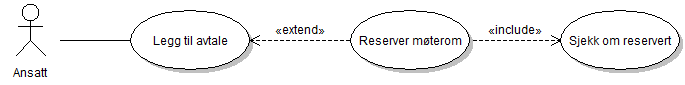
\includegraphics[width=400px]{ucs1.png}
\caption{Use Case-diagram for scenario 1}
\end{figure}

\subsection{Sekvensdiagram}
\begin{figure}[H]
\label{fig:sek1}
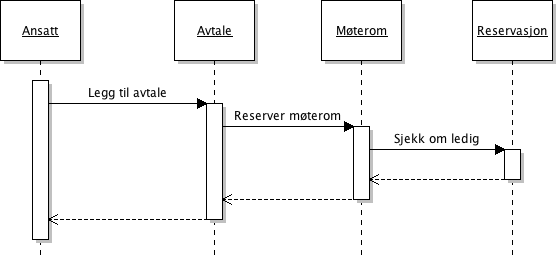
\includegraphics[width=400px]{sekvens1.png}
\caption{Use Case-diagram for scenario 1}
\end{figure}

\newpage
\section{Scenario 2}
\subsection{Use Case}
\begin{figure}[H]
\label{fig:uc2}
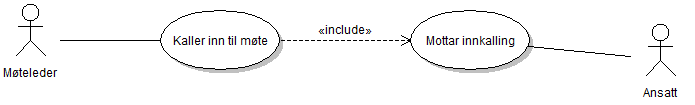
\includegraphics[width=400px]{ucs2.png}
\caption{Use Case-diagram for scenario 2}
\end{figure}

\subsection{Tekstlig Use Case}
\begin{table}[H]
\centering
\label{tab:tuc2}
\begin{tabular}{| l | L{4in} |}
\hline
Use Case & Scenario 2 \\
\hline
Aktør & Møteleder og inviterte ansatte \\
\hline
Trigger & Møteleder inviterer ansatte til et møte \\
\hline
Pre-betingelser & Møteleder har laget møtet \\
\hline
Post-betingelser & Ansatte er invitert til møtet, og mottar melding om dette når de logger seg på systemet. \\
\hline
Normal hendelsesflyt & 
\begin{minipage}{4in}
\vskip 4pt
\begin{itemize}
\item Møteleder opprettet møtet
\item Møteleder inviterer ansatte til møtet
\item Melding blir sendt til de inviterte, som de mottar neste gang de logger seg på
\end{itemize}
\vskip 4pt
\end{minipage}
 \\
\hline
Variasjoner & \\
\hline
Relatert informasjon & De inviterte medlemmene ser meldingen neste gang de logger seg på systemet. \\
\hline
\end{tabular}
\caption{Tekslig Use Case-diagrame}
\end{table}

\subsection{Sekvensdiagram}
\begin{figure}[H]
\label{fig:sek2}
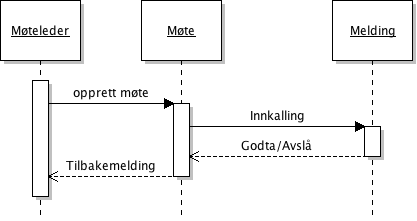
\includegraphics[width=400px]{sekvens2.png}
\caption{Use Case-diagram for scenario 2}
\end{figure}

\newpage
\section{Scenario 3}
\subsection{Use Case}
\begin{figure}[H]
\label{fig:uc3}
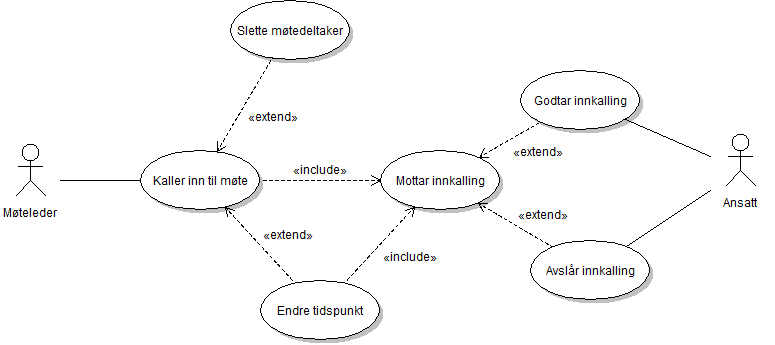
\includegraphics[width=400px]{ucs3.png}
\caption{Use Case-diagram for scenario 3}
\end{figure}

\subsection{Tekstlig Use Case}
\begin{table}[H]
\centering
\label{tab:tuc3}
\begin{tabular}{| l | L{4in} |}
\hline
Use Case & Scenario 3 \\
\hline
Aktør & Møteleder og inviterte ansatte \\
\hline
Trigger & Møteleder inkaller til møte \\
\hline
Pre-betingelser & Brukerene må være logget inn og invitert til samme møte. \\
\hline
Post-betingelser & Møtet blir satt hvor brukerene som har godtatt er invitert og de som har avlyst blir slettet fra møteinkallelsen. \\
\hline
Normal hendelsesflyt & 
\begin{minipage}{4in}
\vskip 4pt
\begin{itemize}
\item Møteleder inkaller til møte
\item Inviterte ansatte mottar møteinkallelse
\item Noen akspeterer møteinkalleslsen og noen avslår møteinkallelsen
\end{itemize}
\vskip 4pt
\end{minipage}
 \\
\hline
Variasjoner & 
\begin{minipage}{4in}
\vskip 4pt
\begin{itemize}
\item Møte blir planlagt på nytt
\item De som avslår møteinkallelsen blir slettet fra møteinkallelsen
\end{itemize}
\vskip 4pt
\end{minipage}
\\
\hline
Relatert informasjon & Alle ansatte som er invitert får beskjed om endringer som blir gjort i møteinkallelsen. \\
\hline
\end{tabular}
\caption{Tekslig Use Case-diagrame}
\end{table}

\subsection{Sekvensdiagram}
\begin{figure}[H]
\label{fig:sek3}
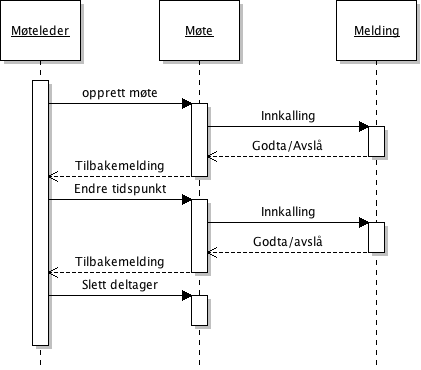
\includegraphics[width=400px]{sekvens3.png}
\caption{Use Case-diagram for scenario 3}
\end{figure}

\newpage
\section{Scenario 4}
\subsection{Tekstlig Use Case}
\begin{table}[H]
\centering
\label{tab:tuc4}
\begin{tabular}{| l | L{4in} |}
\hline
Use Case & Scenario 3 \\
\hline
Aktør & Møteleder og inviterte ansatte \\
\hline
Trigger & Møtelederen avlyser møtet \\
\hline
Pre-betingelser & Møtelederen har laget møtet og invitert andre ansatt. Noen ansatt må også ha godtat møtet. \\
\hline
Post-betingelser & Møten slettes og det gis bedskjed til de involverte ansatt. \\
\hline
Normal hendelsesflyt & 
\begin{minipage}{4in}
\vskip 4pt
\begin{itemize}
\item Møtelederen avlyser møtet.
\item Møtet blir slettet fra Møtelederens personlige kalender.
\item En melding blir sendt til alle inviterte medlemer.
\end{itemize}
\vskip 4pt
\end{minipage}
 \\
\hline
Variasjoner & \\
\hline
Relatert informasjon & De inviterte medlemer ser meldingen neste gang de logger seg på systemet. \\
\hline
\end{tabular}
\caption{Tekslig Use Case-diagrame}
\end{table}

\subsection{Sekvensdiagram}
\begin{figure}[H]
\label{fig:sek4}
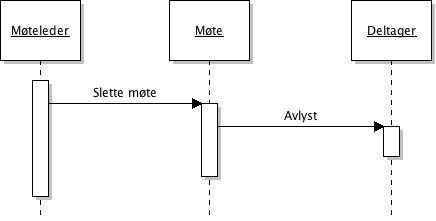
\includegraphics[width=400px]{sekvens4.png}
\caption{Use Case-diagram for scenario 4}
\end{figure}

\newpage
\section{Klassediagram}
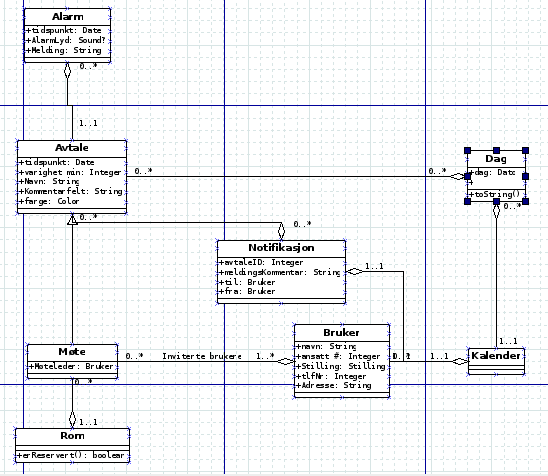
\includegraphics[scale=0.75]{Klassediagram.png}

\newpage
\listoftables

\newpage
\listoffigures

\newpage
\begin{thebibliography}{9}

\bibitem{fpkomp}
	Kompendium til fellesprosjektet,
	\emph{it's learning-gruppa til faget}
\end{thebibliography}

\end{document}
